\documentclass{article}
\usepackage{/Users/jay/LaTeX/cs}
\usepackage{/Users/jay/LaTeX/matlab}

\newcommand{\hmwkClass}{Digital Image Processing, Spring 2018}
\newcommand{\hmwkTitle}{Homework 2}
\newcommand{\hmwkDueDate}{April 11, 2018}
\newcommand{\tb}{\textbf}

\begin{document}

\thispagestyle{empty}
\section*{\hmwkClass \\
    \normalsize{\hmwkTitle} \\
    \normalsize{DUE DATE: \hmwkDueDate}
}

\hfill{Student ID: B03902129 \, Department: CSIE \, Name: Peng-Yu Chen}

% ------ %
% README %
% ------ %

\subsection*{README}

To run my program, simply type \tb{README} in the Command Window of MATLAB application, then it'll run all .m files and output the .raw images.

\begin{lstlisting}[caption = {README.m}]
    % DIP Homework Assignment #2 
    % April 11, 2018
    % Name: Jay Chen
    % ID #: B03902129 
    % email: b03902129@ntu.edu.tw
    
    %#########################################################################
    % Add path first
    %#########################################################################
    
    disp('Add path "./prob1", "./prob2", "./bonus" and "./readwriter"');
    addpath('./prob1');
    addpath('./prob2');
    addpath('./bonus');
    addpath('./readwriter');
    
    %######################################################################### 
    % Problem 1: EDGE DETECTION                                           
    % Implementation 1: 1st order edge detection     
    % Implementation 2: 2nd order edge detection
    % Implementation 3: Canny edge detection
    % Implementation 4: Generate the edge map by avoiding obtaining edges of
    %                   the noise
    % M-files: prob1.m, edgeDetectFirst.m, edgeDetectSecond.m and
    %                   edgeDetectCanny.m
    % Output: None
    % Usage: run prob1 to call other .m files
    %#########################################################################
    
    fprintf('----------------------------------------\n');
    fprintf('Running "prob1"\n----------------------------------------\n');
    prob1();
    
    %######################################################################### 
    % Problem 2: GEOMETRICAL MODIFICATION                                           
    % Implementation 1: Perform edge crispening, I3 -> C         
    % Implementation 2: Design a warping function, C -> D
    % M-files: prob2.m
    % Usage: run prob2 to call other .m files
    % Output: None
    % Parameters:
    %       * 3 x 3 Low Pass Filter: b = 1, 2, 3, ..., 30
    %       * n x n Square Median Filter: window size = 3, 5, 7, ..., 15
    %       * n + n - 1 Cross Median Filter: cross size = 3, 5, 7, ..., 15
    %       * Wrinkle remover: threshold = 3
    %                          crossMedianFilter with cross size = 15
    %#########################################################################
    
    fprintf('----------------------------------------\n');
    fprintf('Running "prob2"\n----------------------------------------\n');
    prob2();
    
    %######################################################################### 
    % Bonus                                           
    % Implementation 1: Design an algorithm to enhance images
    % M-files: bonus.m
    % Usage: run bonus to call other .m files
    % Output: None
    %#########################################################################
    
    fprintf('----------------------------------------\n');
    fprintf('Running "bonus"\n----------------------------------------\n');
    bonus();    
\end{lstlisting}

\newpage
% ---------------------------- %
% PROBLEM 1: IMAGE ENHANCEMENT %
% ---------------------------- %
\subsection*{PROBLEM 1: EDGE DETECTION}

\begin{enumerate}[label=(\alph*)]

    \item Given an image $I_1$ as show in Fig. 1(a), please perform $1^\text{st}$ order edge detection, $2^\text{nd}$ order edge detection, and Canny edge detection to obtain corresponding edge maps. Please describe each method in detail, specify each parameter clearly and discuss how each of them affects the resultant edge map. What are pros and cons of each method? [Please output the edge points with intensity value $1$ and background points with intensity value $0$.]

    \subsubsection*{$1^\text{st}$ Order Edge Detection}

    Since the given image is discrete, we have to use approximation method. There are three approximation implementations in my program, and all of them need to calculate the gradient value $G$ for each entry $(i, j)$ in the given image first. \\

    We do this by computing the row gradient ($G_x$) and the column gradient ($G_y$) separately, then take the squrae root of the summation of $G_x^2$ and $G_y^2$ to obtain $G$)

    \begin{enumerate}[label=(\roman*)]
        \item 3 points
        \begin{align*}
            G_x(i, j) & = I(i, j) - I(i, j - 1) \\
            G_y(i, j) & = I(i, j) - I(i + 1, j) \\
            G(i, j) & = \sqrt{G_x^2(i, j) + G_y^2(i, j)}
        \end{align*}

        \item 4 points
        \begin{align*}
            G_x(i, j) & = I(i, j) - I(i + 1, j + 1) \\
            G_y(i, j) & = I(i, j + 1) - I(i + 1, j) \\
            G(i, j) & = \sqrt{G_x^2(i, j) + G_y^2(i, j)}
        \end{align*}

        \item 9 points

        If using the Prewitt Mask, then we set $k = 1$. \\
        If using the Sobel Mask, then we set $k = 2$.

        \begin{align*}
            A_0 & = I(i - 1, j - 1) \\
            A_1 & = I(i - 1, j) \\
            A_2 & = I(i - 1, j + 1) \\
            A_3 & = I(i, j + 1) \\
            A_4 & = I(i + 1, j + 1) \\
            A_5 & = I(i + 1, j) \\
            A_6 & = I(i + 1, j - 1) \\
            A_7 & = I(i, j - 1) \\
            G_x(i, j) & = \frac{1}{k + 2}[(A_2 + kA_3 + A_4) - (A_0 + kA_7 + A6)] \\
            G_y(i, j) & = \frac{1}{k + 2}[(A_0 + kA_1 + A_2) - (A_6 + kA_5 + A4)] \\
            G(i, j) & = \sqrt{G_x^2(i, j) + G_y^2(i, j)}
        \end{align*}
    \end{enumerate}

    \newpage
    After calculating the $G$. We have to do thresholding. We can pick threshold $T$ by examine the cumulative distribution function. \\

    If $G(i, j) \ge T$, then we set the corresponding entry $(i, j)$ as an edge point (intensity value = 1); otherwise ($G(i, j) < T$), we set the corresponding entry $(i, j)$ as a non-edge point (intensity value = 0). \\

    The resultant images are in the next page. \\

    Here we use $p$ denoting how many $points$ our approximation method used, $T$ to denote what $threshold$ we select, and in the case of $p = 9$, we have another parameter $k$ to decide whether we use Prewitt Mask ($k = 1$) or Sobel Mask ($k = 2$). \\

    \begin{itemize}
        \item When $T$ is equal to $10$, no matter what approximation method we applied, the result is not good, since there are still too many noises in the images. 

        \item When $T$ grows up to $30$, the result becomes much better, and we can now see more stripes in our palm images.

        \item When $T$ grows up to $50$, the result is less detailed then $T = 30$ since the thresholding filter out too many non-noisy entries.
    \end{itemize}

    As we can see, the parameter $p$ doesn't affect the result so much. I think this is because that in first order, no matter how many points we use to calculate the $G_x$ and $G_y$, we can still get the similar magnitude $G$. \\

    Of course, the parameter $T$ seriously affects the result. We can analyze the statistics of the magnitude (histogram) to see this. \\

    Finally, the parameter $k$ seems to influence the image in a distinct way. We compare images (h) and (k) in the next page, which have the same parameters $p = 9$ and $T = 30$ but different $k$, and we can see that when $k = 2$, the background it's much cleaner then when $k = 1$. But on the other hand, when we compare images (i) and (l), it seems that when $k = 2$, it sacrifices too many details in order to get a cleaner background.

    \begin{figure}
        \centering
        \begin{subfigure}[b]{0.3\textwidth}
            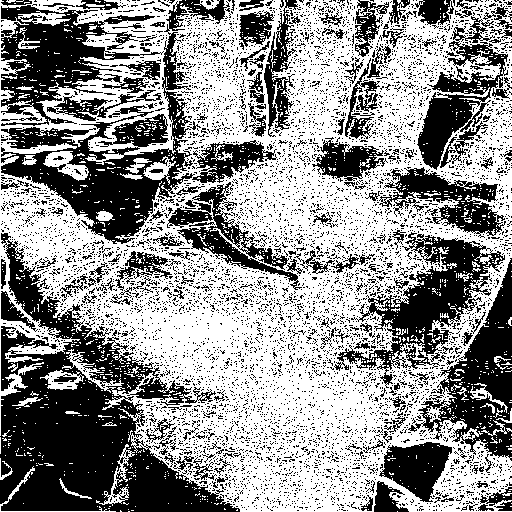
\includegraphics[width=\textwidth]{img/ED1_3_10.png}
            \caption{$p = 3$, $T = 10$}
        \end{subfigure}
        ~
        \begin{subfigure}[b]{0.3\textwidth}
            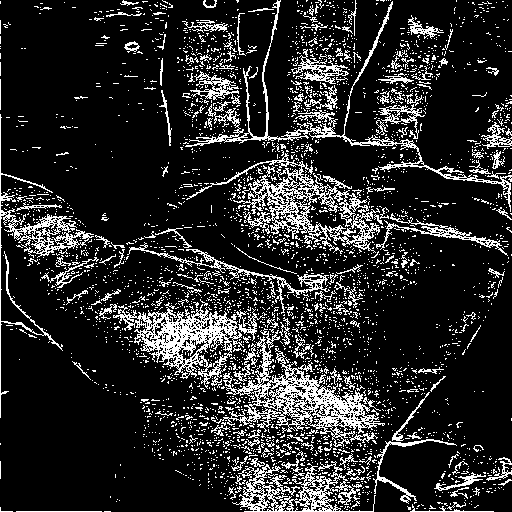
\includegraphics[width=\textwidth]{img/ED1_3_30.png}
            \caption{$p = 3$, $T = 30$}
        \end{subfigure}
        ~
        \begin{subfigure}[b]{0.3\textwidth}
            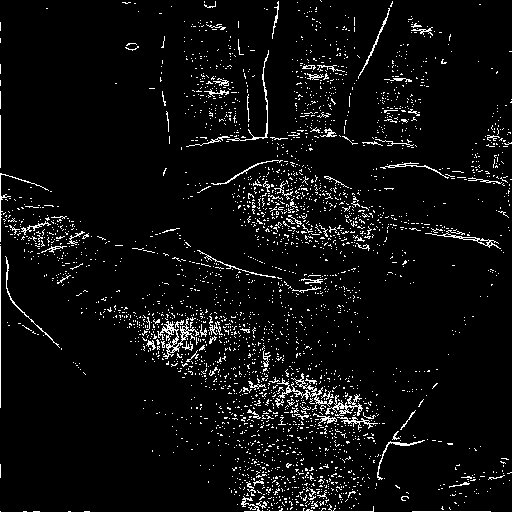
\includegraphics[width=\textwidth]{img/ED1_3_50.png}
            \caption{$p = 3$, $T = 50$}
        \end{subfigure}
        
        % newline
        
        \begin{subfigure}[b]{0.3\textwidth}
            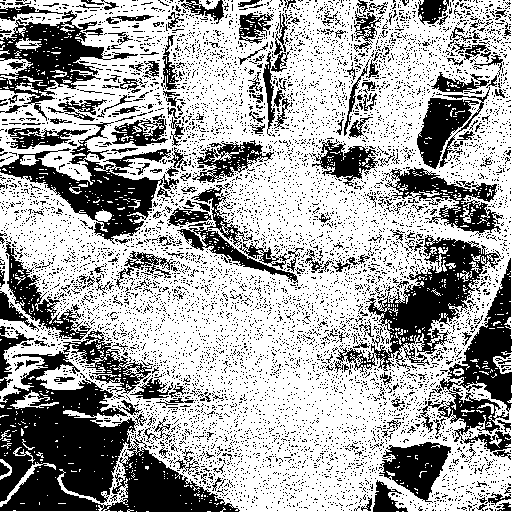
\includegraphics[width=\textwidth]{img/ED1_4_10.png}
            \caption{$p = 4$, $T = 10$}
        \end{subfigure}
        ~
        \begin{subfigure}[b]{0.3\textwidth}
            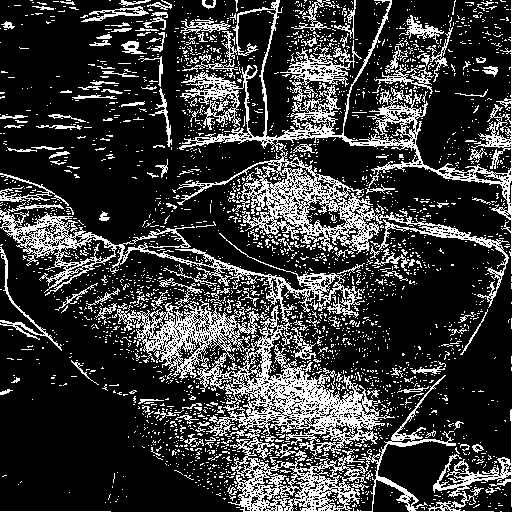
\includegraphics[width=\textwidth]{img/ED1_4_30.png}
            \caption{$p = 4$, $T = 30$}
        \end{subfigure}
        ~
        \begin{subfigure}[b]{0.3\textwidth}
            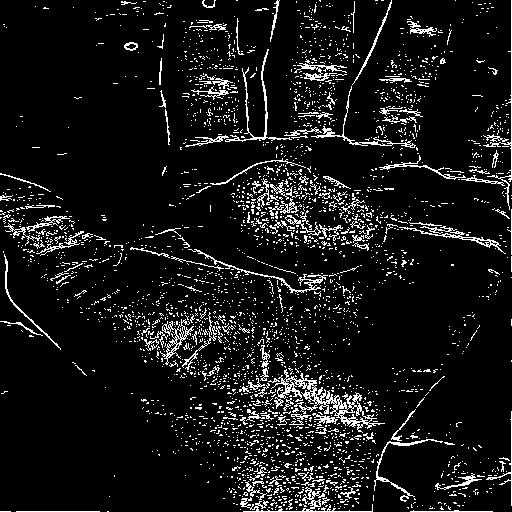
\includegraphics[width=\textwidth]{img/ED1_4_50.png}
            \caption{$p = 4$, $T = 50$}
        \end{subfigure}
        
        % newline    
        
        \begin{subfigure}[b]{0.3\textwidth}
            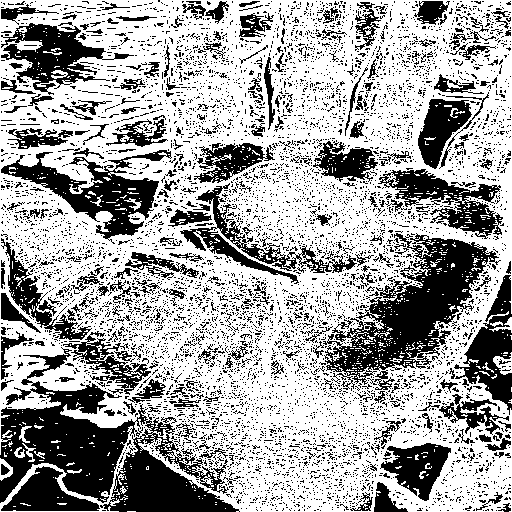
\includegraphics[width=\textwidth]{img/ED1_9_10_1.png}
            \caption{$p = 9$, $T = 10$, $k = 1$}
        \end{subfigure}
        ~
        \begin{subfigure}[b]{0.3\textwidth}
            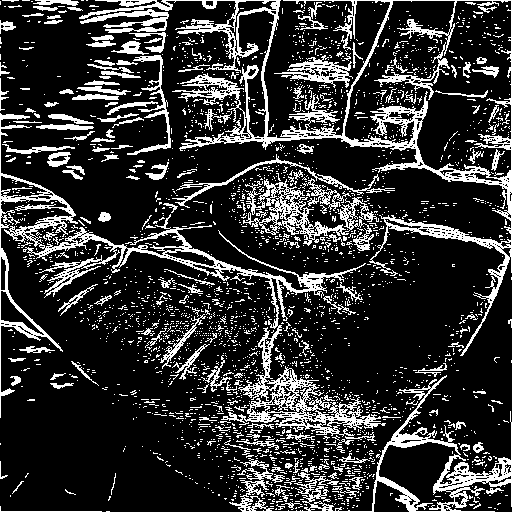
\includegraphics[width=\textwidth]{img/ED1_9_30_1.png}
            \caption{$p = 9$, $T = 30$, $k = 1$}
        \end{subfigure}
        ~
        \begin{subfigure}[b]{0.3\textwidth}
            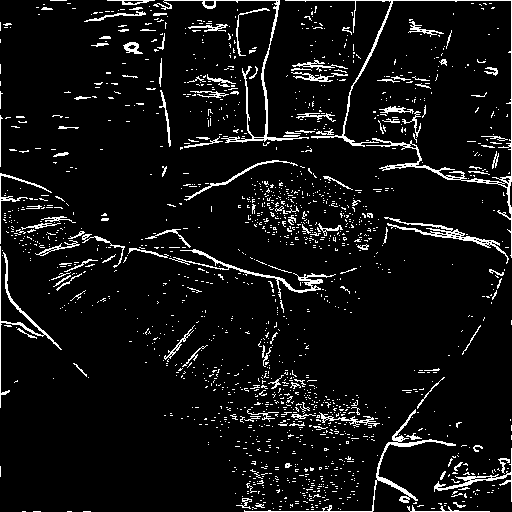
\includegraphics[width=\textwidth]{img/ED1_9_50_1.png}
            \caption{$p = 9$, $T = 50$, $k = 1$}
        \end{subfigure}
        
        % newline    

        \begin{subfigure}[b]{0.3\textwidth}
            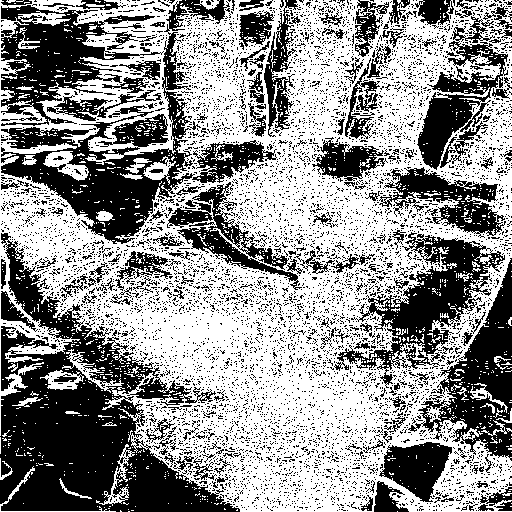
\includegraphics[width=\textwidth]{img/ED1_3_10.png}
            \caption{$p = 3$, $T = 10$, $k = 2$}
        \end{subfigure}
        ~
        \begin{subfigure}[b]{0.3\textwidth}
            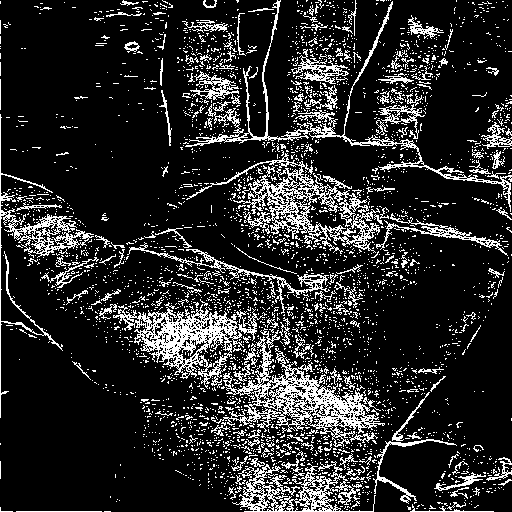
\includegraphics[width=\textwidth]{img/ED1_3_30.png}
            \caption{$p = 3$, $T = 30$, $k = 2$}
        \end{subfigure}
        ~
        \begin{subfigure}[b]{0.3\textwidth}
            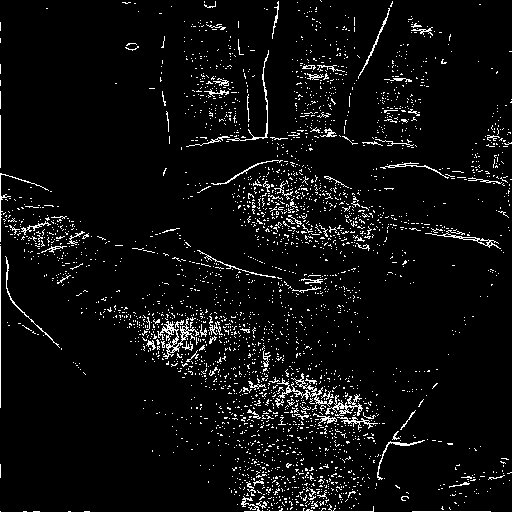
\includegraphics[width=\textwidth]{img/ED1_3_50.png}
            \caption{$p = 3$, $T = 50$, $k = 2$}
        \end{subfigure}
        
        \caption{1st Order Edge Detection with different parameters $point$, $threshold$ and $k$}
    \end{figure}

    \newpage
    \subsubsection*{$2^\text{nd}$ Order Edge Detection}

    To perform $2^\text{nd}$ Order Edge Detection, we first need to pad the array, then do the filtering, Here I choose the following two masks:

    $$
    \frac{1}{4} 
    \begin{bmatrix}
        0 &  1 & 0 \\
        1 & -4 & 1 \\
        0 &  1 & 0
    \end{bmatrix} \text{(four-neighbor)} \qquad
    \frac{1}{8}
    \begin{bmatrix}
        -1 & -1 & -1 \\
        2 &  2 &  2 \\
        -1 & -1 & -1
    \end{bmatrix} \text{(eight-neighbor)}
    $$

    Like $1^\text{st}$ Order Edge Detection, we have to decide a threshold $T$ to filter out unnecessary entries.

    Finally, we have to do zero-crossing detection for each $I(i, j) = 0$. \\

    We can see that when moving to $2^\text{nd}$ Order Edge Detection, the whiteness becomes less than which in the $1^\text{st}$ Order Edge Detection, and overall the effect is not good. However, image (a) still provides a clear view of the edge despite the fact that it's noisy.

    \begin{figure}[!htb]
        \centering
        \begin{subfigure}[b]{0.3\textwidth}
            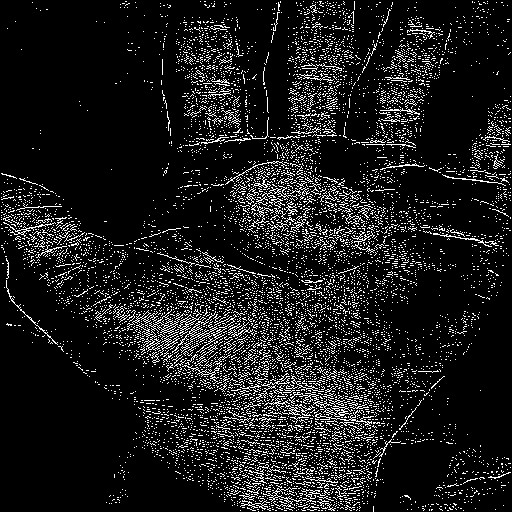
\includegraphics[width=\textwidth]{img/ED2_4_10.png}
            \caption{$n = 4$, $T = 10$}
        \end{subfigure}
        ~
        \begin{subfigure}[b]{0.3\textwidth}
            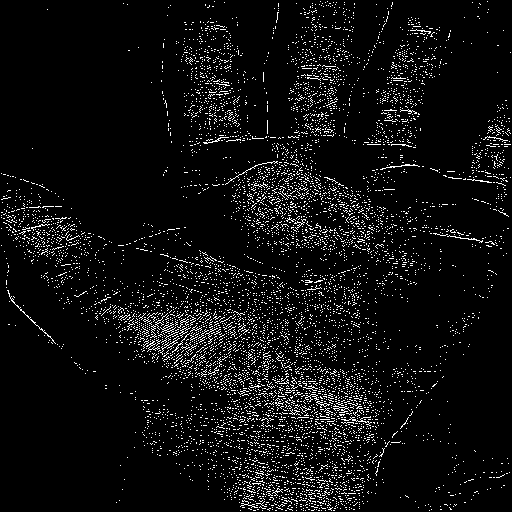
\includegraphics[width=\textwidth]{img/ED2_4_15.png}
            \caption{$n = 4$, $T = 15$}
        \end{subfigure}
        ~
        \begin{subfigure}[b]{0.3\textwidth}
            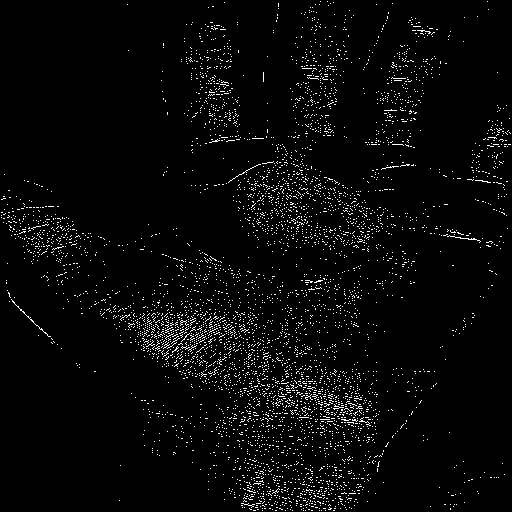
\includegraphics[width=\textwidth]{img/ED2_4_20.png}
            \caption{$n = 4$, $T = 20$}
        \end{subfigure}
        
        % newline    

        \begin{subfigure}[b]{0.3\textwidth}
            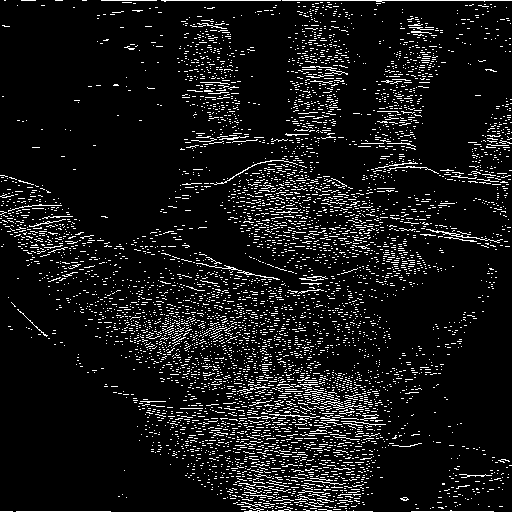
\includegraphics[width=\textwidth]{img/ED2_8_10.png}
            \caption{$n = 8$, $T = 10$}
        \end{subfigure}
        ~
        \begin{subfigure}[b]{0.3\textwidth}
            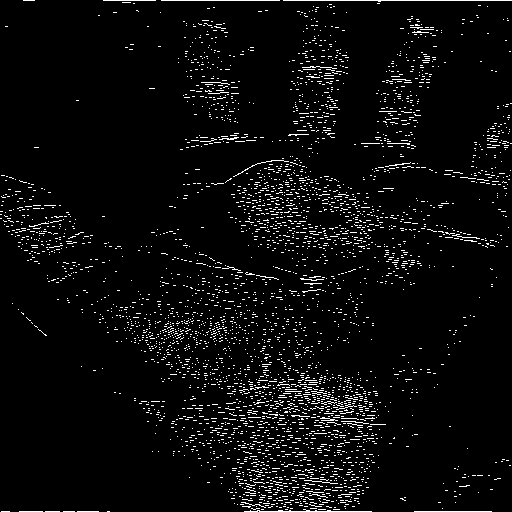
\includegraphics[width=\textwidth]{img/ED2_8_15.png}
            \caption{$n = 8$, $T = 15$}
        \end{subfigure}
        ~
        \begin{subfigure}[b]{0.3\textwidth}
            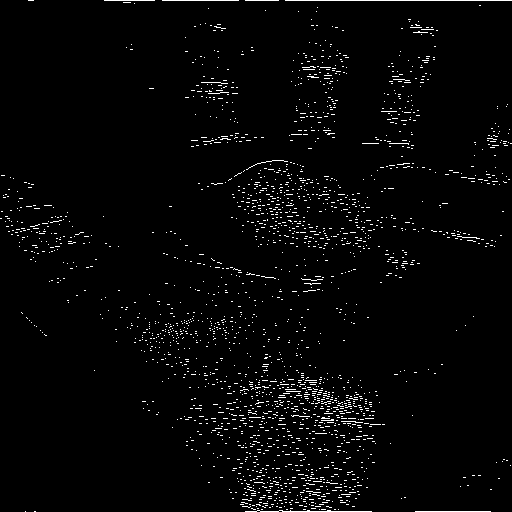
\includegraphics[width=\textwidth]{img/ED2_8_20.png}
            \caption{$n = 8$, $T = 20$}
        \end{subfigure}

        \caption{2nd Order Edge Detection with different parameters $n$ and $threshold$}
    \end{figure}

    \newpage
    \subsubsection*{Canny Edge Detection}

    There are five steps in the Canny Edge Detection algorithm:

    \begin{enumerate}
        \item [1.] \tb{Noise reduction}
        
        We first smooth the image with a Gaussian filter by the following $5 \times 5$ mask:

        $$
        \frac{1}{159} 
        \begin{bmatrix}
            2 &  4 &  5 &  4 & 2 \\
            4 &  9 & 12 &  9 & 4 \\
            5 & 12 & 15 & 12 & 5 \\
            4 &  9 & 12 &  9 & 4 \\
            2 &  4 &  5 &  4 & 2
        \end{bmatrix}
        $$

        \item [2.] \tb{Compute gradient magnitude and orientation}

        Then we compute the gradient magnitude by doing $1^\text{st}$ Order Edge Detection with parameter $p = 9$, $T = 30$ and $k = 2$ (Sobel Mask). 
        
        Also we compute the orientation by calculating $$\theta(i, j) = \tan^{-1} \Bigg(\frac{G_y(i, j)}{G_x(i, j)}\Bigg)$$

        \item [3.] \tb{Non-maximal suppression}

        We do non-maximal suppression by searching the nearest neighbors $(i', j')$ and $(i'', j'')$ along the edge normal.

        $$
        G_N(i, j) =
        \begin{cases}
            G(i, j) & \text{ if } G(i, j) > G(i', j') \text{ and } G(i, j) > G(i'', j'') \\
            0       & \text{ otherwise }
        \end{cases}
        $$

        \item [4.] \tb{Hysteretic thresholding}

        Then we label each pixels according to two thresholds: $T_H$ and $T_L$

        $$
        \begin{cases}
            G_N(i, j) \ge T_H & \text{Edge Pixel} \\
            T_H > G_N(i, j) \ge T_L & \text{Candidate Pixel} \\
            G_N(i, j) < T_L & \text{Non-edge Pixel}
        \end{cases}
        $$

        \item [5.] \tb{Connected component labeling method}

        Finally, we declare the connected componet if a candidate pixel is connected to an edge pixel directly or via another candidate pixel.
    \end{enumerate}

    \newpage

    In this problem, we set $T_L = 0.075$ and $T_H = 0.175$.

    We can see that after doing the Gaussian filter, the image becomes smooth.
    
    Computing gradient can preliminarily outline the image.
    
    Non-maximal method, also known as thinning algorithm can make the edge thinner to remove unnecessary conflict.

    Hysteretic thresholding can help us labeling the desired and candidate edges.

    Finally, by applying connected component labeling method, we can obtain the image produced by Canny Edge Detection.

    \begin{figure}[!htb]
        \centering
        \begin{subfigure}[b]{0.3\textwidth}
            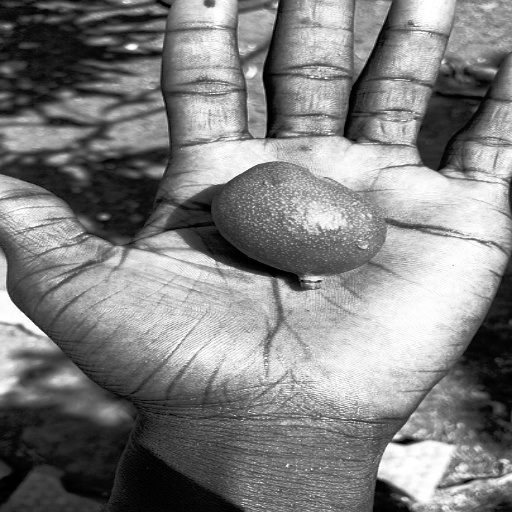
\includegraphics[width=\textwidth]{img/I1.png}
            \caption{sample1.raw}
        \end{subfigure}
        ~
        \begin{subfigure}[b]{0.3\textwidth}
            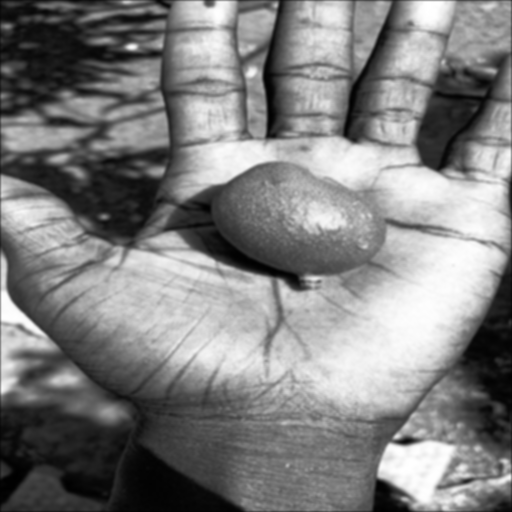
\includegraphics[width=\textwidth]{img/GF.png}
            \caption{Step 1: Gaussian filter}
        \end{subfigure}
        ~
        \begin{subfigure}[b]{0.3\textwidth}
            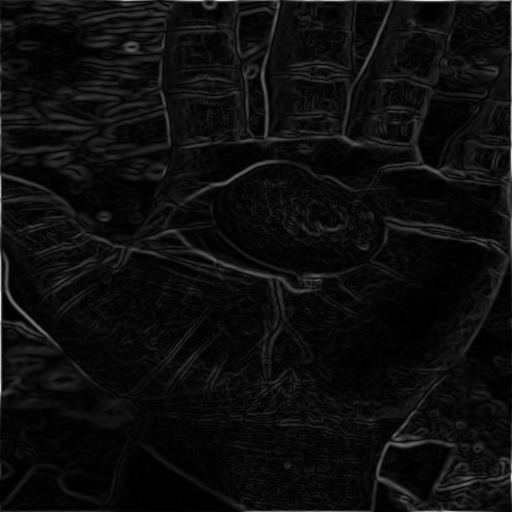
\includegraphics[width=\textwidth]{img/G.png}
            \caption{Step 2: Magnitude}
        \end{subfigure}
        
        % newline    

        \begin{subfigure}[b]{0.3\textwidth}
            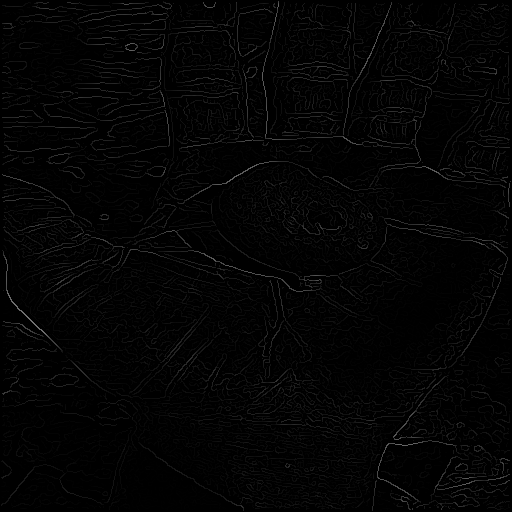
\includegraphics[width=\textwidth]{img/GN.png}
            \caption{Step 3: Non-maximal}
        \end{subfigure}
        ~
        \begin{subfigure}[b]{0.3\textwidth}
            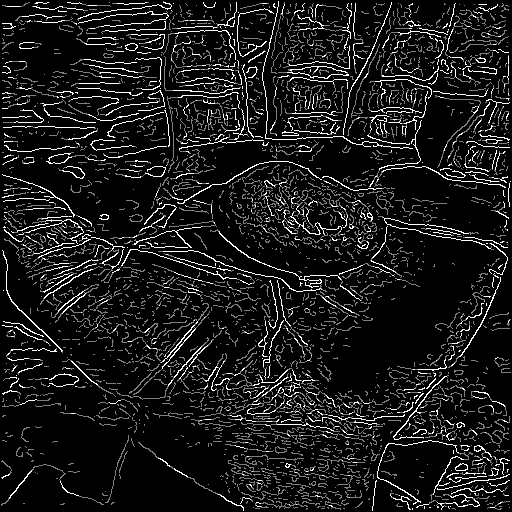
\includegraphics[width=\textwidth]{img/CC.png}
            \caption{Step 4: Hysteretic}
        \end{subfigure}
        ~
        \begin{subfigure}[b]{0.3\textwidth}
            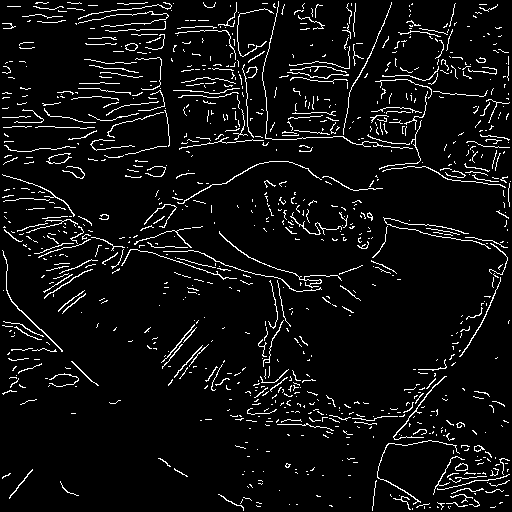
\includegraphics[width=\textwidth]{img/E.png}
            \caption{Step 5: Connected component}
        \end{subfigure}

        \caption{Steps of Canny Edge Detection}
    \end{figure}

    \newpage

    \item Given an image $I_2$ with periodic noise as shown in Fig. 1(b), please design your own method to generate the edge map by avoiding obtaining edges of the noise. [Please output the edge points with intensity value $1$ and background points with intensity value $0$.] \\

    The steps are same as above, the only difference is that here I set the $T_L = 0.175$ and $T_L = 0.225$ because the frequency of sample2.raw is higher than sample1.raw.

    \begin{figure}[!htb]
        \centering
        \begin{subfigure}[b]{0.3\textwidth}
            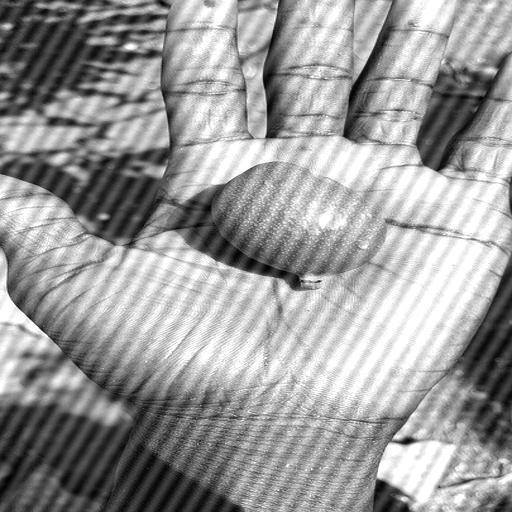
\includegraphics[width=\textwidth]{img/I2.png}
            \caption{sample2.raw}
        \end{subfigure}
        ~
        \begin{subfigure}[b]{0.3\textwidth}
            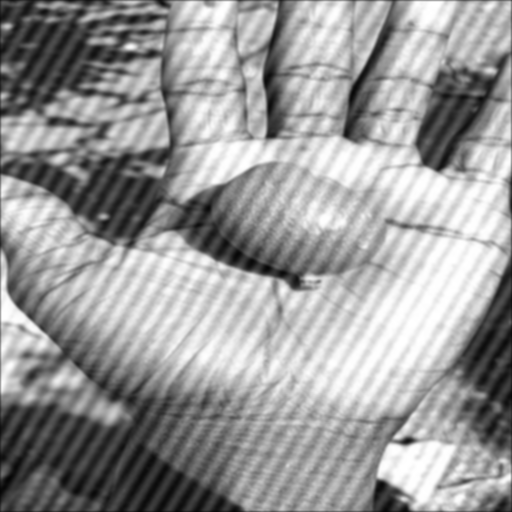
\includegraphics[width=\textwidth]{img/GF(noise).png}
            \caption{Gaussian filter}
        \end{subfigure}
        ~
        \begin{subfigure}[b]{0.3\textwidth}
            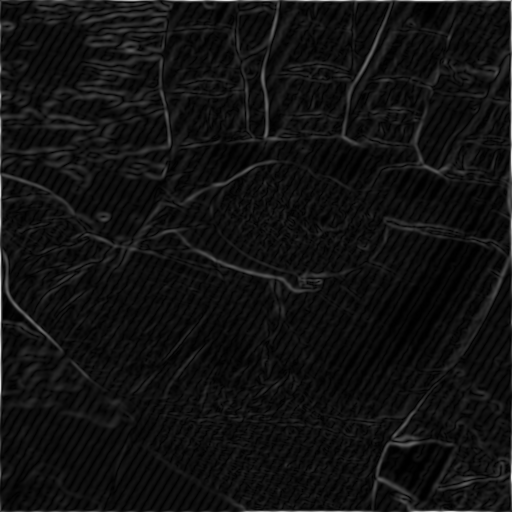
\includegraphics[width=\textwidth]{img/G(noise).png}
            \caption{Magnitude}
        \end{subfigure}
        
        % newline    

        \begin{subfigure}[b]{0.3\textwidth}
            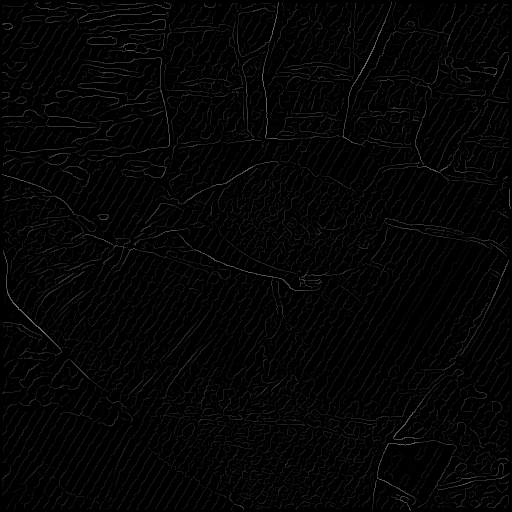
\includegraphics[width=\textwidth]{img/GN(noise).png}
            \caption{Non-maximal}
        \end{subfigure}
        ~
        \begin{subfigure}[b]{0.3\textwidth}
            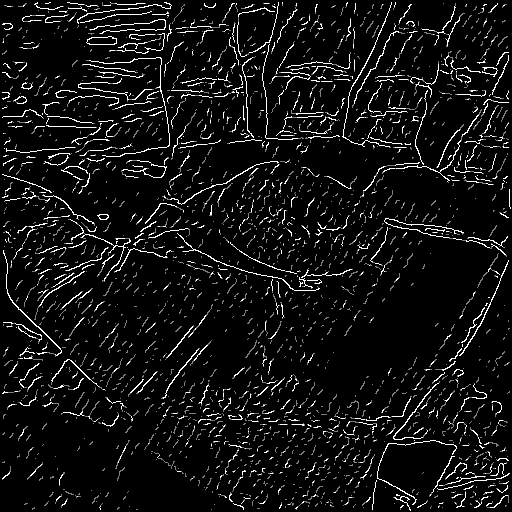
\includegraphics[width=\textwidth]{img/C(noise).png}
            \caption{Hysteretic}
        \end{subfigure}
        ~
        \begin{subfigure}[b]{0.3\textwidth}
            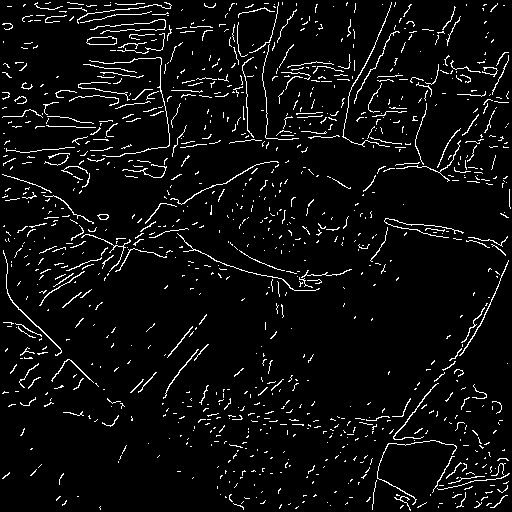
\includegraphics[width=\textwidth]{img/E(noise).png}
            \caption{Connected component}
        \end{subfigure}
    \end{figure}
\end{enumerate}

\newpage
% ----------------------------------- %
% PROBLEM 2: GEOMETRICAL MODIFICATION %
% ----------------------------------- %
\subsection*{PROBLEM 2: GEOMETRICAL MODIFICATION}

Given an image $I_3$ as shown in Fig. 2(a).

\begin{enumerate}[label=(\alph*)]
    \item Please perform edge crispening on $I_3$ and denote the result as $C$. Show the parameters adopted and provide some discussions on the result as well.

    We perform Edge Crispening by calculating $E = \frac{c}{2c - 1} I - \frac{1 - c} {2c - 1} L \cdot I$ with different parameter $L$ and $c$.

    We can see that $L$ doesn't influence the result so much, but $c$ does influence it because it's the key parameter to adjust the filter.

    \begin{figure}[!htb]
        \centering
        \begin{subfigure}[b]{0.3\textwidth}
            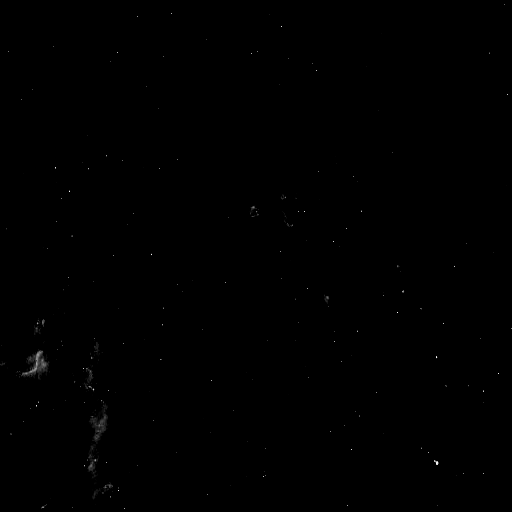
\includegraphics[width=\textwidth]{img/C_5_06.png}
            \caption{$L = 5$, $c = 0.6$}
        \end{subfigure}
        ~
        \begin{subfigure}[b]{0.3\textwidth}
            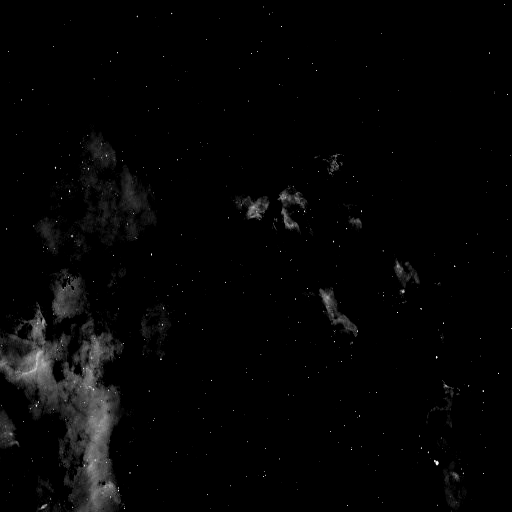
\includegraphics[width=\textwidth]{img/C_5_07.png}
            \caption{$L = 5$, $c = 0.7$}
        \end{subfigure}
        ~
        \begin{subfigure}[b]{0.3\textwidth}
            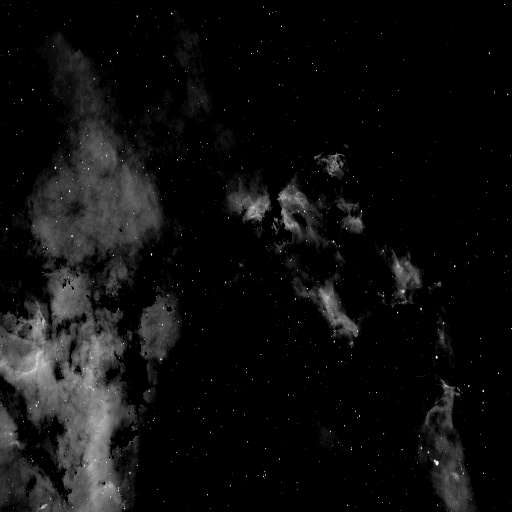
\includegraphics[width=\textwidth]{img/C_5_08.png}
            \caption{$L = 5$, $c = 0.8$}
        \end{subfigure}
        
        % newline    

        \begin{subfigure}[b]{0.3\textwidth}
            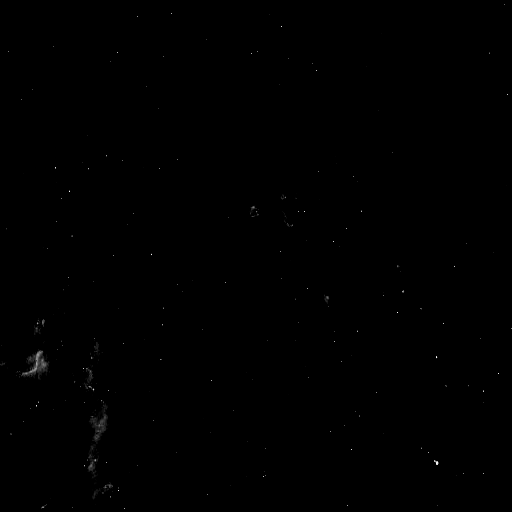
\includegraphics[width=\textwidth]{img/C_7_06.png}
            \caption{$L = 7$, $c = 0.6$}
        \end{subfigure}
        ~
        \begin{subfigure}[b]{0.3\textwidth}
            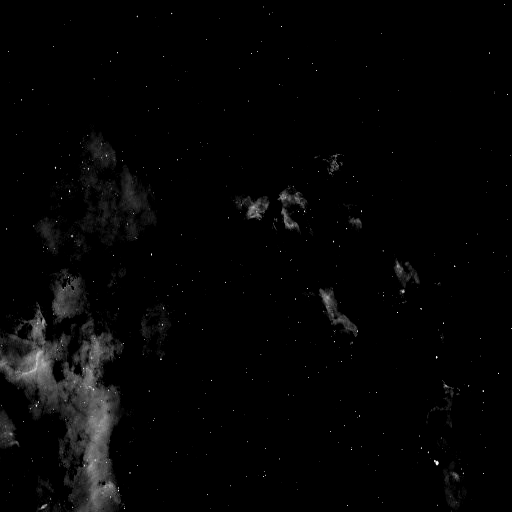
\includegraphics[width=\textwidth]{img/C_7_07.png}
            \caption{$L = 7$, $c = 0.7$}
        \end{subfigure}
        ~
        \begin{subfigure}[b]{0.3\textwidth}
            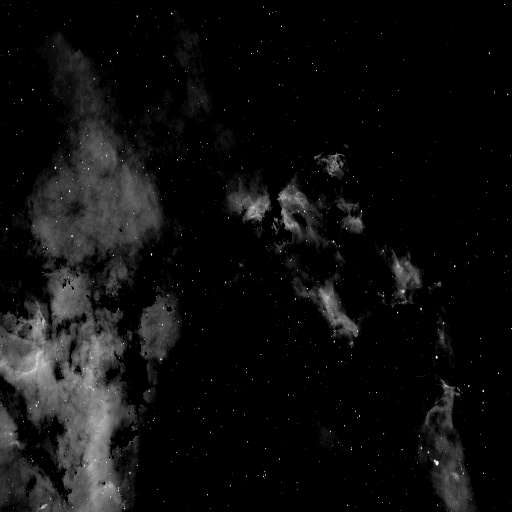
\includegraphics[width=\textwidth]{img/C_7_08.png}
            \caption{$L = 7$, $c = 0.8$}
        \end{subfigure}

        % newline    

        \begin{subfigure}[b]{0.3\textwidth}
            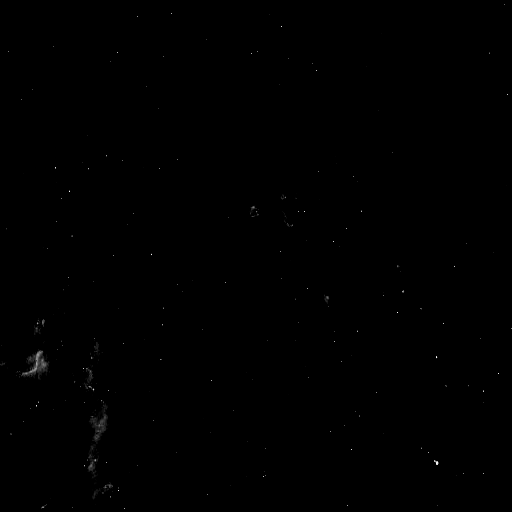
\includegraphics[width=\textwidth]{img/C_9_06.png}
            \caption{$L = 9$, $c = 0.6$}
        \end{subfigure}
        ~
        \begin{subfigure}[b]{0.3\textwidth}
            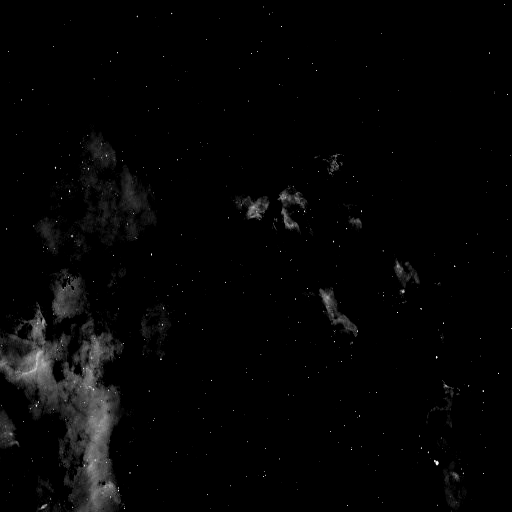
\includegraphics[width=\textwidth]{img/C_9_07.png}
            \caption{$L = 9$, $c = 0.7$}
        \end{subfigure}
        ~
        \begin{subfigure}[b]{0.3\textwidth}
            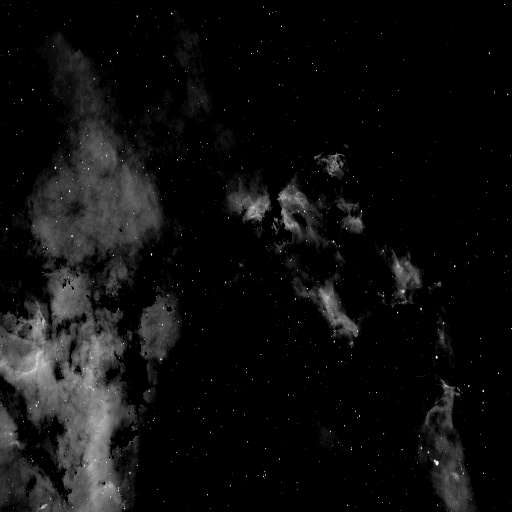
\includegraphics[width=\textwidth]{img/C_9_08.png}
            \caption{$L = 9$, $c = 0.8$}
        \end{subfigure}
        \caption{Edge Crispening with different parameters $L$ and $c$}
    \end{figure}

    \newpage
    \item Please design a warping function to convert the image $C$ to image $D$ with a shape similar to Fig. 2(b).

    I use the following formula to calculate the warping image:
    \begin{align*}
        x & = i + 20\sin((j - 10) / 24) \\
        y & = j + 18\sin((i + 40) / 40)
    \end{align*}

    \begin{figure}[!htb]
        \centering
        \begin{subfigure}[b]{0.3\textwidth}
            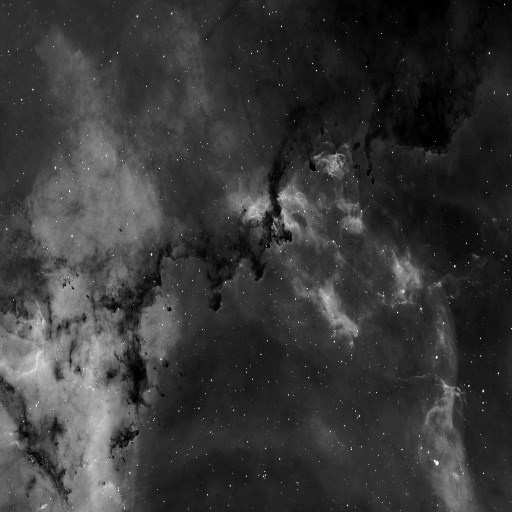
\includegraphics[width=\textwidth]{img/C.png}
            \caption{sample2.raw}
        \end{subfigure}
        ~
        \begin{subfigure}[b]{0.3\textwidth}
            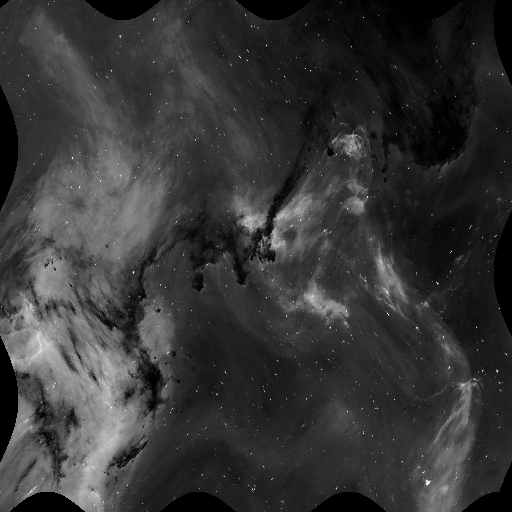
\includegraphics[width=\textwidth]{img/D.png}
            \caption{warped image}
        \end{subfigure}
        \caption{Perform warping function}
    \end{figure}
\end{enumerate}

\newpage
% ----- %
% BONUS %
% ----- %
\subsection*{BONUS}

Please design an algorithm to enhance the following two images as best as you can. The top 10\% students will get the extra credit. \\

I use edge crispening to enhance the image:

$$E = \frac{c}{2c - 1} I - \frac{1 - c}{2c - 1}L \cdot I.$$

The parameter are $c = 0.8$ and $L = 7$. After doing the edge crispening, the enhanced images become much more detailed than the original one.

\begin{figure}[!htb]
    \centering
    \begin{subfigure}[b]{0.3\textwidth}
        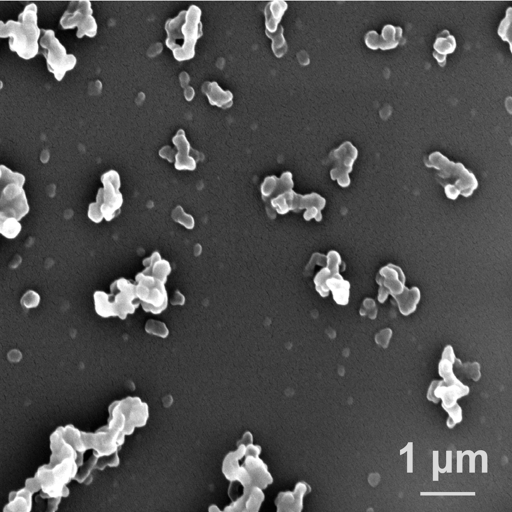
\includegraphics[width=\textwidth]{img/I4.png}
        \caption{sample4.raw}
    \end{subfigure}
    ~
    \begin{subfigure}[b]{0.3\textwidth}
        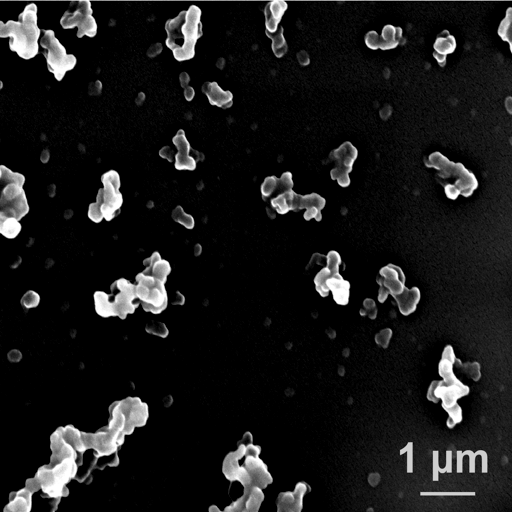
\includegraphics[width=\textwidth]{img/I4_EC.png}
        \caption{sample4.raw enhanced}
    \end{subfigure}

    % newline

    \begin{subfigure}[b]{0.3\textwidth}
        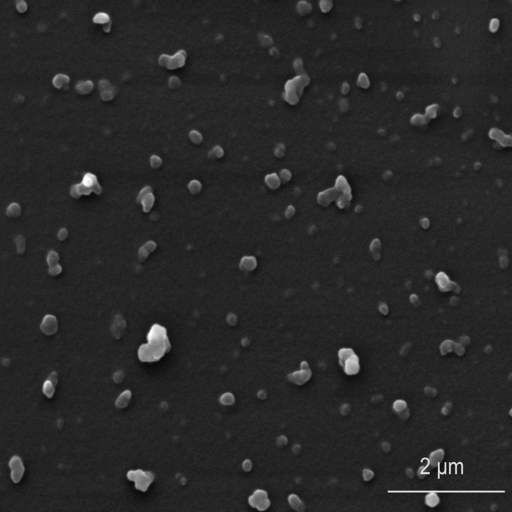
\includegraphics[width=\textwidth]{img/I5.png}
        \caption{sample5.raw}
    \end{subfigure}
    ~
    \begin{subfigure}[b]{0.3\textwidth}
        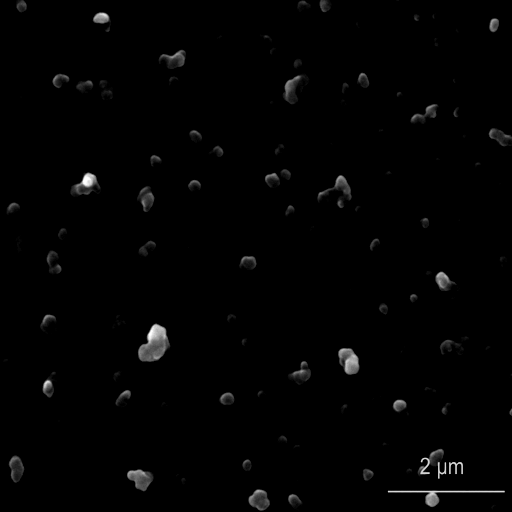
\includegraphics[width=\textwidth]{img/I5_EC.png}
        \caption{sample5.raw enhanced}
    \end{subfigure}
    \caption{Enhanced images}
\end{figure}



\end{document}